\section{Test de interconexión de red Zybo}
\hypertarget{TestConexion}{}
\subsection{Descripción}
Una vez se han conectado todos los dispositivos al switch como se indicó en el tutorial de creación de una infraestructura de red de placas Zybo, y, estando encendidos todos los dispositivos, necesitamos comprobar que existe conexión entre todos ellos.

Para ello, se ha desarrollado un script en bash, llamado \texttt{Inicio.sh}, que comprueba el estado de conexión de los dispositivos. En este script se pueden definir las tarjetas Zybo que se vayan a usar, con su alias y su dirección IP de red (previamente establecida). Para ello, tendremos que abrir el fichero \texttt{Inicio.sh} con nuestro editor favorito y cambiar las siguientes líneas:
\begin{figure}[h]
	\centering
	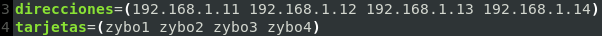
\includegraphics[scale=0.7]{Anexos/Anexo2/Test/Script.png}
	\caption{Líneas a modificar en el script.}
	\label{Líneas a modificar en el script}
\end{figure}

\textcolor{red}{Esta foto hay que cambiarla debido a un cambio en las IP's. Pero eso lo haré cuando tenga las tarjetas que me dejé en Madrid.}
\begin{itemize}
	\item \textbf{Línea 3:} Introducir la dirección IP de la tarjeta que queramos añadir. O borrar la que queramos quitar.
	\item \textbf{Línea 4:} Introducir el alias de la tarjeta que queramos añadir. O borrar la que queramos quitar.
\end{itemize}

El script será ejecutado desde el ordenador central abriendo una terminal en el directorio donde se ubique el mismo. Este script lo podemos encontrar en el anexo \hyperlink{ScriptConexion}{Inicio.sh}.

Cabe destacar que tiene dos modos de funcionamiento:
\subsubsection{Normal}
En esta opción, la salida del script será meramente informativa, devolviendo si la tarjeta está o no conectada a la red.
\begin{itemize}
	\item Se ejecuta mediante el comando:
	\begin{center}
		\texttt{./Inicio.sh}
	\end{center}
	\item El script lanza cuatro paquetes de ping a cada una de las tarjetas, una por una, guardando el resultado del mismo comando en una variable y sin mostrarla por pantalla.
	\item Mediante scraping\footnote{Técnica usada mediante programas software para extraer información de un texto.} el script lee la salida del último de los paquetes de ping.
	\item \textbf{Éxito:} Si en dicho texto no se encuentra la secuencia ``\texttt{100\% packet loss}'' indicará que la tarjeta está conectada.
	\item \textbf{Fracaso:} Si en dicho texto se encuentra la secuencia ``\texttt{100\% packet loss}'' indicará que la tarjeta a la cual se está realizando el ping, no está conectada.
\end{itemize}

\subsubsection{Verboso}
En esta opción, la salida del script es más detallada ya que muestra más información al respecto de la conexión.

\begin{itemize}
	\item Se ejecuta mediante el comando:
	\begin{center}
		\texttt{./Inicio.sh -v}
	\end{center}
	\item El script lanza cuatro paquetes de ping a cada una de las tarjetas, una por una.
	\item Mediante la opción \texttt{-v} le indicamos que nos muestre por pantalla la salida de los comandos de ping, para ver el estado de la conexión más detalladamente.
\end{itemize}

%\section{Script}
%El script está programado en bash y su nombre es \texttt{Inicio.sh}.
%
%%\newpage
%\subsubsection{Diagrama de flujo}
%\begin{figure}[h]
%	\centering
%	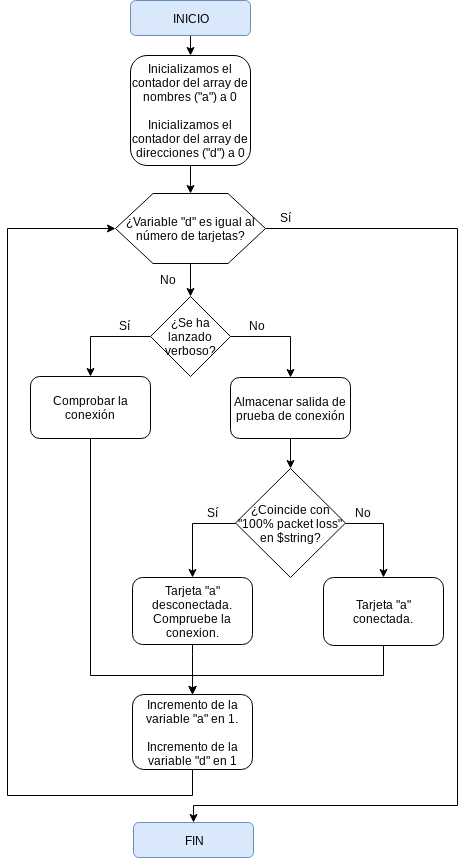
\includegraphics[scale=0.562]{Anexos/Anexo2/Test/Inicio.png}
%	\caption{Diagrama de flujo de \texttt{Inicio.sh}}
%	\label{Diagrama de flujo de Inicio.sh}
%\end{figure}
%
%\newpage
%\subsubsection{Código}
%\lstinputlisting[language=Bash]{Anexos/Anexo2/Test/Inicio.sh}
%\begin{center}
%	Código de \texttt{Inicio.sh} usando cuatro tarjetas como ejemplo.
%\end{center}
%
%\textcolor{red}{No se si es mejor hacerlo así o poner todos los códigos con su correspondiente diagrama de flujo en el apéndice C que es el que he dejado exclusivamente para los códigos.}
